\section{Generation dispatch and price coordination}\label{sec:generation}

\subsection{An hourly convex supply model}
Let $b_t$ be background demand and $L_t$ fleet energy in one-hour intervals.
With linear marginal costs $a_{it}$, generator limits $\bar g_{it}$, and
declared initial outputs $g_{i0}$, define
\begin{equation}\label{eq:dispatch-value}
\begin{aligned}
 H(d)=\min_g\quad &\sum_{i,t}a_{it}g_{it},\\
 \text{subject to}\quad &\sum_i g_{it}=d_t,\quad
 0\le g_{it}\le\bar g_{it},\\
 &-R^-_{it}\le g_{it}-g_{i,t-1}\le R^+_{it}.
\end{aligned}
\end{equation}
Piecewise-linear or convex quadratic production costs give analogous convex
models. The incremental supply cost is $G(L)=H(b+L)-H(b)$, identified with
$F$ in Section~\ref{sec:model}. The baseline is fixed across alternatives.
Balance multipliers are marginal prices; ramps couple their determination
across time. This hourly model follows the dispatch-price interpretation of
\citet{scaglione2016marginal}, without claiming to reproduce that paper's
continuous-time trajectory model. No generator commitment binaries or
network congestion are included. Nodal balances and transmission constraints
would require depot-specific loads and locational prices.

All physical fleet loads in the example below are supply-feasible. More
generally, capacity limits require an explicit supply-feasible deviation set
or a specified backup-supply rule. Extending a cost as $+\infty$ cannot
silently change which fleet alternatives are admissible. A generation LP
may have several optimal balance multipliers. Report a selected price and,
when testing existence of support, consider the full declared admissible
price set. One solver-selected price alone cannot exclude the others.

\subsection{What dual coordination does and does not imply}
Dualize $L=e(x)$ in joint fleet and supply planning. With
$V(p)=\min_{x\in\Fleet}\{c(x)+p^\top e(x)\}$, the dual is
\begin{equation}\label{eq:dispatch-dual}
 \max_p Q(p),\qquad Q(p)=V(p)-G^*(p).
\end{equation}
Under Proposition~\ref{prop:theory-support}'s qualification its value is
$CH$, so the physical primal--dual gap is exactly $D-CH$. This is the
classical convex-hull pricing connection \citep{gribikHoganPope2007}.
\citet{alizadeh2016coupled} coordinate convex traffic flows and power
dispatch through dual prices. Replacing those divisible flows by an atomic
complete-fleet oracle retains a concave dual but need not retain zero
physical duality gap. Complete-schedule column generation provides another
route to the same convexification \citep{andrianesis2022hull}.

At $p_k$, let $x_k$ globally minimize the fleet objective and let $s_k$
maximize $p_k^\top s-G(s)$. Then $e(x_k)-s_k$ is a supergradient of $Q$,
and a projected ascent step is
\begin{equation}\label{eq:dispatch-update}
 p_{k+1}=\Pi_P\{p_k+\alpha_k[e(x_k)-s_k]\}.
\end{equation}
Suppose a closed convex price region $P$ contains an unrestricted dual
optimizer $p^*$, the oracles attain their optima, and the supergradient norms
are at most $M$ along the run. The projection inequality gives
\begin{equation}\label{eq:dispatch-rate}
 Q(p^*)-\max_{1\le k\le K}Q(p_k)
 \le\frac{\|p_1-p^*\|^2+M^2\sum_{k=1}^K\alpha_k^2}
 {2\sum_{k=1}^K\alpha_k}.
\end{equation}
Thus $\alpha_k\propto k^{-1/2}$ gives a best-dual-value guarantee of order
$\log K/\sqrt K$. It does not alone prove convergence of each price
iterate, a unique limiting price, or a physical fleet. A price restriction
excluding all unrestricted optimizers instead solves a different dual.
An inexact fleet incumbent is not an exact supergradient oracle.

A balanced fleet and supply response at one common price would attain
both primal and dual values and force $D=CH$. A positive gap therefore
excludes a balanced joint limit of exact responses at a finite limiting
price. It does not imply that every schedule sequence must switch forever:
a tie rule can repeatedly choose one fleet at a hull price while its load
still differs from the supply response. The undamped gradient-reset cycle
in Figure~\ref{fig:exact-cycle} is a different update from
\eqref{eq:dispatch-update}.

For the quadratic construction, we ran \eqref{eq:dispatch-update} for
20,000 analytic oracle calls, starting at $(6,4)$, projecting onto
$\R_+^2$, and taking $\alpha_k=0.5/\sqrt k$. All continuous two-bus
charging choices are minimized analytically; fleet ties select one bus.
Before call 20,000, the price is approximately $(5.3412,4.6588)$, the
current dual is 94.8300, and the best dual so far is 94.887499, compared
with exact $CH=94.8875$. The one-bus frequency is 0.6682 versus the hull
weight 0.675; the step-weighted frequency is 0.6603. The last 60 responses
contain 38 bus-count switches. Figure~\ref{fig:dual-replay} distinguishes
current from best dual bounds. These are cheap analytic calls and finite-run
diagnostics, not 20,000 timetable MIPs or a proof of primal convergence.

\begin{figure}[t]
\centering
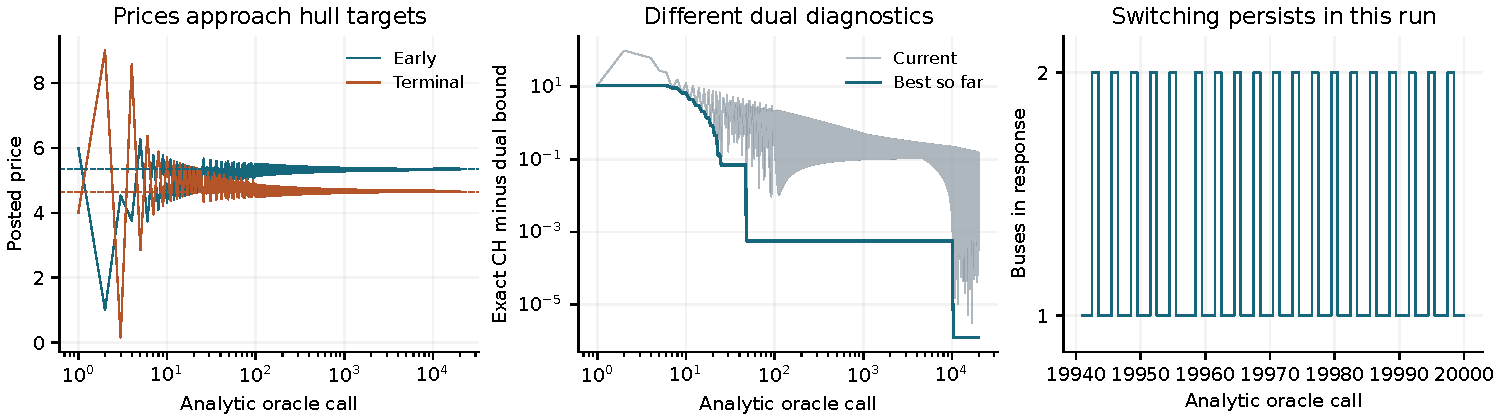
\includegraphics[width=\linewidth]{figures/quadratic_dual_replay.pdf}
\caption{Projected dual ascent on the existing quadratic two-service
example, with the declared initialization and step sizes. Dashed lines are
the exact hull-price coordinates. A nearly optimal best dual bound coexists
with changing physical responses and a less accurate current dual bound.}
\label{fig:dual-replay}
\end{figure}

\subsection{An exact two-generator example with hourly ramps}
Keep every fleet constraint and continuous charging choice from
Section~\ref{sec:exact}. Generation now spans the consecutive hours
$[1,2]$, $[2,3]$, and $[3,4]$: the fleet load is
$L=(x,0,30-x)$ and background demand is $b=(0,15,0)$. The middle hour,
when service B operates, cannot be omitted from an hourly ramp model.
Both generators start at zero; no terminal generation level is imposed.
Costs are declared synthetic hourly offers, with no fixed commitment costs.
Generator A has marginal costs $(7,5,1)$ and capacities $(10,15,15)$;
generator B has costs $(6,5,5)$ and capacities $(10,15,30)$.
A's initial upward limit is 10 and its two subsequent hourly upward limits
are 5. All downward limits and B's upward limits are 30. Power and energy
numbers coincide in these one-hour intervals.

Background supply costs $H(b)=75$. Let $a,m,z$ denote A's early, middle
and terminal outputs. On the full feasible fleet interval $0\le x\le10$,
subtracting the baseline leaves $150+x+a-4z$. The two ramps and terminal
capacity imply $z\le\min(15,a+10)$, attained with $m=a+5$ for every
$a\in[0,x]$. Minimizing over $a$ therefore gives the exact supply value
\begin{equation}\label{eq:ramp-value}
 G(x,0,30-x)=
 \begin{cases}110-2x,&0\le x\le5,\\95+x,&5\le x\le10.\end{cases}
\end{equation}
The one-bus plan costs $7+G(10,0,20)=112$; the best two-bus plan costs
$14+G(5,0,25)=114$. The complete-fleet hull retains the operating-cost
boundary $14-0.7x$, giving
\begin{equation}\label{eq:ramp-gap}
 D_G=112,\qquad CH_G=\frac{221}{2}=110.5,\qquad D_G-CH_G=\frac32.
\end{equation}
The minimizing mixture gives equal weight to the one-bus load $(10,0,20)$
and the two-bus load $(0,0,30)$. At its mean $(5,0,25)$, dispatch is
A $=(5,10,15)$ and B $=(0,5,10)$, with both of A's hourly upward ramps
binding (Figure~\ref{fig:ramp-example}).

At that mean the exact set of balance prices is
$p=(s,5,5)$, $3\le s\le6$. Positive B output fixes the last two prices;
A's stationarity gives equal ramp rents $7-s$ and terminal-capacity rent
$s-3$, while B's unused early output requires $s\le6$. Selecting
$p^*=(5.7,5,5)$ makes the two supporting fleet plans tie at private cost
164. Its generator dual supplies the global cut
$G(L)\ge(p^*)^\top L-53.5$, tight at the mean. Thus the dual lower bound
is $164-53.5=110.5$, equal to the mixture upper bound. This derivation is
independent of the quadratic example's prices.

The physical one-bus optimum has the unique dispatch price $(6,5,5)$ and
regret 3. The physically feasible two-bus plan at the kink $x=5$ instead
has a price-dependent regret: $32-5s$ for $3\le s\le5.7$, and $5s-25$
for $5.7\le s\le6$. Its smallest admissible regret is 3.5, attained at
$s=5.7$, equal to its physical cost minus $CH_G$. This illustrates why a
nonsmooth supply model needs a declared price selection or a test over
the admissible set.

Relaxing only A's two inter-hour upward limits from 5 to 30 gives
$G_0(x,0,30-x)=90+x$. Both the physical and hull minima then equal 104,
attained by the two-bus plan with $x=0$. These controlled synthetic cases
isolate the change in the supply constraints; they are not measurements of
price-support failure in a public timetable. Small LP solutions independently
check dispatch, balance prices and hull values, while the affine branch
derivation and rational dual certificate establish the exact claims.

\begin{figure}[t]
\centering
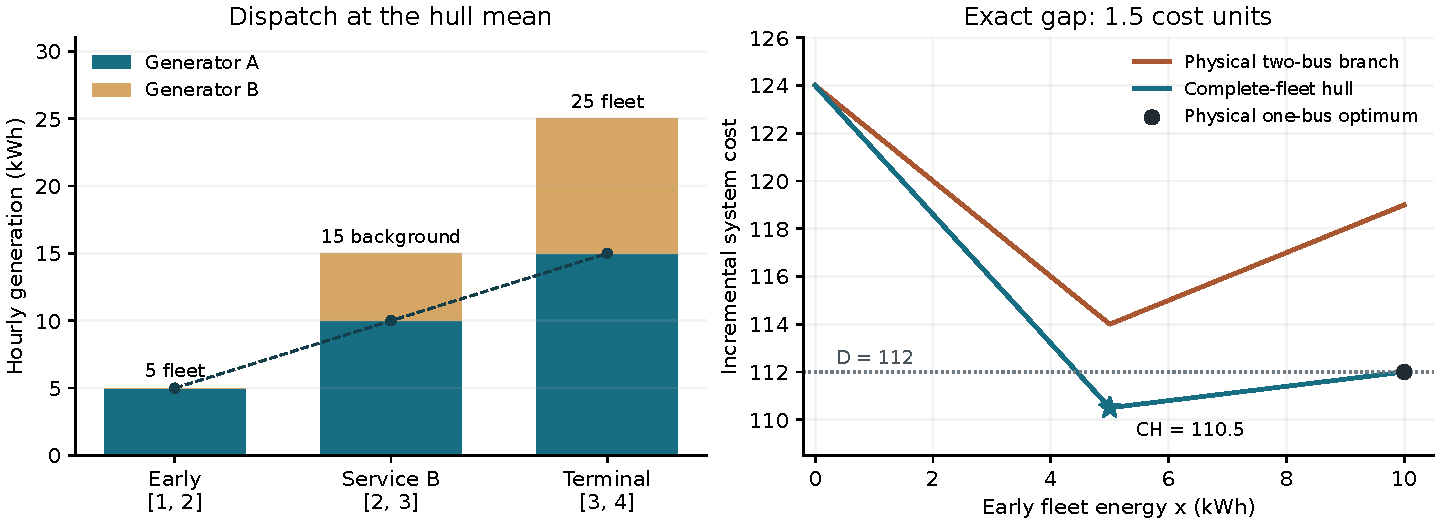
\includegraphics[width=\linewidth]{figures/ramped_generation_example.pdf}
\caption{The hourly generation example. Left: generation serving the hull
mean; the middle hour serves only background demand, and A rises by its
5-unit limit in each interval. Right: physical two-bus and hull costs over
the full continuous charging interval, with the one-bus optimum marked
separately. All costs and offers are synthetic.}
\label{fig:ramp-example}
\end{figure}

